% \section{Data Presentation and Analysis}
\specialsection{Data Presentation and Analysis}{}{black}{white}

\subsection{Quantitative Findings}

\subsection{Release early, release often}


\subsubsection{Trends in Git Commits}


% \subsubsection{Patterns in Forum Contributions}

% Although Ben Fry remains the most active contributor in forum discussions, the activity distribution is more balanced compared to Git commits. This may be due to the broader range of topics discussed, including technical issues and bugs.
% A total of 1039 people posted on the forum in that time period. There were core people there that were actively participating as can be seen in the ~ref{processing-alpha-dot}

% Casey Reas “I would say that the period from around 2002 to 2006 was one when it felt almost like a unified international community created around the forum.” ([“Graphic design in the post-digital age: a survey of practices fueled by creative coding”, 2021, p. 331](zotero://select/library/items/GKA2GIS5)) ([pdf](zotero://open-pdf/library/items/QL4IRL3M?page=333&annotation=BRCSCF56))

% \begin{figure}[h!] 
%   \centering
%   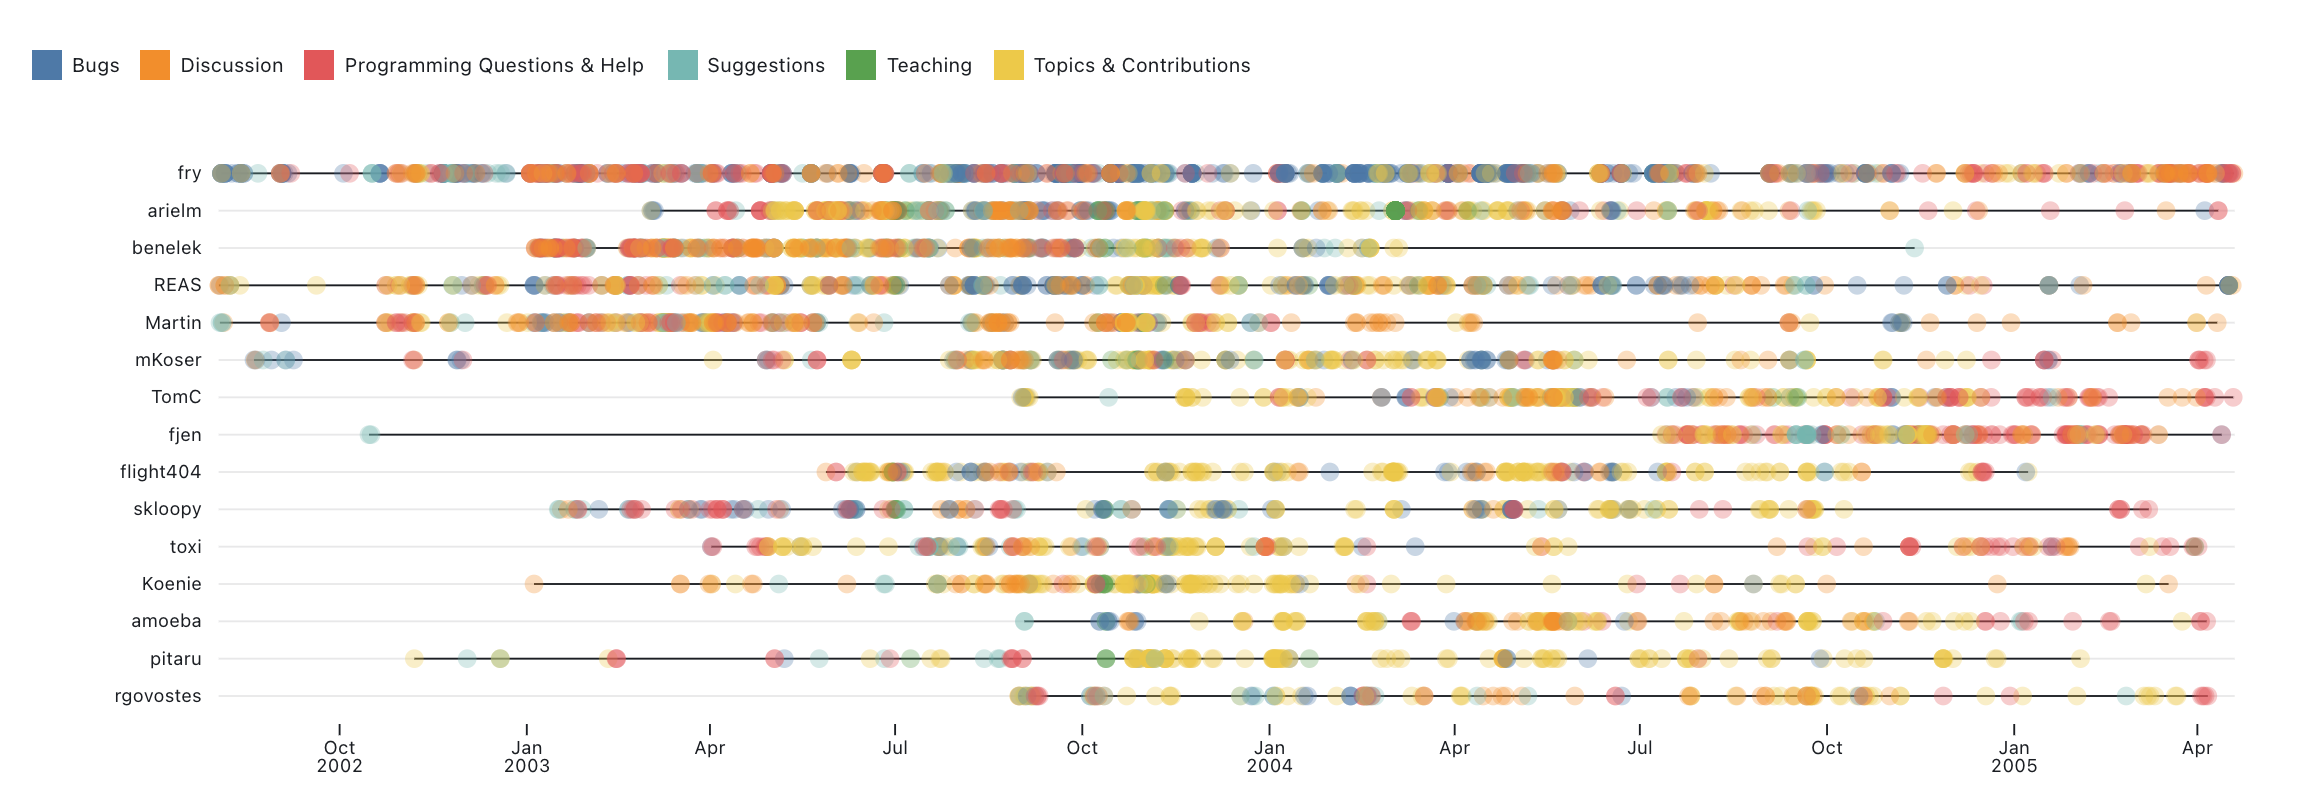
\includegraphics[width=0.9\textwidth]{images/alpha-forum-top15.png} 
%   \caption{Posting of 15 most active contributors on the alpha forum}
%   \label{fig:processing-alpha-dot}
% \end{figure}

% “"Given enough eyeballs, all bugs are shallow." I dub this: "Linus's Law."” ([Raymond, 1999, p. 29](zotero://select/library/items/87U5FDLI)) ([pdf](zotero://open-pdf/library/items/UZP875I7?page=7&annotation=89BX42PF))
% While this didn't translate well to the number of code contributors, we can see an incresed activity in the forum adjacent to releases suggesting that people contribute to at least finding bugs as seen in ~ref{figure:forum-git-activity}

\subsubsection{Patterns in Forum Contributions}

